\documentclass[leqno]{article}
\usepackage[left=0.5in,right=0.5in]{geometry}
\usepackage[utf8]{inputenc}
\usepackage{amsmath, amsfonts, color, booktabs, centernot, graphicx, fancyhdr}
\setlength\parindent{0pt}
\begin{document}
\title{Notes on CS70 Discussion Solutions CrowdSourcing Model}
\author{Leah Dickstein}

\maketitle

\section{Background}
Gireeja wrote a paper creating/defining a model for Crowd Sourcing. The CS70 Discussion Solutions is a situation that closely matches the model.\\

\section{Questions}
What is it about the situation that caused it to match a crowdsourcing model? (What criterion defined it as a crowdsourcing problem?)\\
How can we improve the contest so it better fits the goal of the manager? If we change 1 parameter, what will happen? Let's tweak parameters in controlled experiments (changing 1 variable at a time) and see how and by how much parameters affect the outcomes of the contest. Then, let's design the ideal contest for admin and discussion solutions. Let's also observe how students react to different contests to determine how they are learning and what learning styles best suit them.\\

\subsection{How can we do this?}
We create a model that mathematizes the utility the manager gets and explore parameters to increase that utility. \\

\subsection{Hypothesis}
\begin{itemize}
\item All pay auction: students must bid attempted solutions regardless if they get the reward (extra credit) or not
\item TRUE discussion solutions are never posted online, only student solutions 
\end{itemize}

\section{Description}
\textbf{Players}: Students\\
\textbf{Incentive}: Extra Credit (\textcolor{red}{Is prize value relatively unknown to students? They don't know HOW much extra credit they get until they bid and win for the first time.})\\
\textbf{Manager}: Professor, GSIs, Readers = admin\\
\textbf{Incentive/Goal for Manager}: Get the right discussion solutions and get maximum number of students to learn by participating \emph{with effort.} A third possible goal is to differentiate who the strongest players are.\\
\textbf{Cost of prize to manager}: Virtually nothing if we consider grade inflation to be minimal, thus Utility = value of function f($\overrightarrow{x}$).\\

\subsection{Motivations to bid}
\begin{enumerate}
\item Participation grade
\item Need of extra credit
\item Internal incentive
\begin{enumerate}
\item Wanted the practice so why not post for a chance at reward
\item Enjoy doing problems
\item Want attention from readers/GSIs \textcolor{red}{(weak/maybe nonexistent)}
\end{enumerate}
\end{enumerate}

\subsection{Costs}
\begin{itemize}
\item TIME! HIGH cost because of need to LaTeX or equivalent
\begin{enumerate}
\item Almost all students submitted LaTeX versions instead of scanned in solutions. This is because if you're selected you must submit LaTeX solutions, so why not submit LaTeX from the get-go?
\item LaTeX solutions are perceived as more professional and thus more likely to be selected for reward
\end{enumerate}
\item It needs to be 100\% complete and correct, which could be a deterrent. Students feel they can't meet the threshold.
\item Other classes compete for attention
\item Low reward. Most students would rather study for tests with large impact. The word "extra" makes the prize feel unnecessary, and many students are so overworked they only focus on what's necessary to pass classes. Students who are already acing the course and have leftover time feel no \emph{need} for "extra" credit. Some students are irrational and value video games/reddit/short term pleasures over extra credit, because they fail to see/appreciate the value of extra credit.
\end{itemize}

\section{Comparison}
\subsection{Differences with Gireeja's model}
\begin{enumerate}
\item Players do NOT know each other's strengths
\begin{itemize}
\item However, based on their grades, they know relatively where they are in the class
\item Since it's Berkeley/maybe people in general, many players assume they are "bad" compared to everyone else (\textcolor{red}{assumption??})
\end{itemize}
\item In model, there was a Nash equilibrium where only 2 players bid. Players 3 through n of less strength bid 0 with probability 1. In the current setting 3 people get extra credit, so there should be 3 to 4 players who bid.
\end{enumerate}

\subsection{Connection to Gireeja's paper}
The task is a combination of a selective task and market creation. It's selective because there's a "right" answer to solutions. Even if students post different ways of approaching the problem, there's still a "correct end goal." It's market creation because the managers want as many people to participate as possible with effort, so the more students that participate the better.\\

For selective task, $U_task = max(x_1,x_2,\dots x_n) - A$
\[ \mathbb{E}[U_task] = \frac{A}{6}\left(\frac{3c_2+c_1}{c_2^2}\right) - A \]
This expected utility is positive iff $\frac{3c_2-c_1}{6c_2^2} - 1 > 0$\\
If $c_2 \gg c_1$ then $c_2 < \frac{1}{2}$\\
If $3c_2-c_1 = \epsilon$ is small (low difference) then $c_2^2 < \frac{\epsilon}{6}$ ensures positive utility\\
This is based on $c_1 < c_2$\\

For market creation, $f(\overrightarrow{x}) = \alpha n + \beta$\\
Manager utility doesn't depend on utility of players at all

\subsection{What this means}
If the managers gave everyone extra credit simply for participating, everyone would only put in the minimal bid. This is why the manager wants participation \emph{with effort.} The manager wants to challenge everyone.\\

Since there are elements of both selective task and market creation in the Discussion Solutions situation, we need to decide which one is weighted more and/or how to combine the two to create a model for this scenario.

\section{Data}
\begin{tabular}{c c l}
Discussion & \# of bids & Players\\
1B & 4 bids & Hansong Zhang, Kevin Chen, Daniel Suryakusuma, Andrew Luo\\
2A & 5 bids & Viraj Mahesh, Lingtian Cheng, Hansong Zhang, Hongling Lu, Arnav Dugar\\
2B & 5 bids & Lingtian Cheng, Hongling Lu, Melanie Cebula, Myra Haqqi, Arnav Dugar\\
3A & 5 bids & Hongling Lu, Viraj Mahesh, Brian Chu, Myra Haqqi, Arnav Dugar\\
3B & 4 bids & Chris Dock, Hansong Zhang, Hongling Lu, Myra Haqqi\\
4A & 4 bids & Kevin Mawhorter, Hongling Lu, Melanie Cebula, Cong Chen\\
4B & 5 bids & Arnav Dugar, Anurag Ajay, Myra Haqqi, Hongling Lu, Lingtian Cheng\\
5A & 0 bids & Midterm so no solution thread posted\\
5B & 6 bids & Hongling Lu, Arnav Dugar, Aditya Challa, Anurag Ajay, Myra Haqqi, Alex Yang\\
6A & 4 bids & Arnav Dugar, Hongling Lu, Myra Haqqi, Aditya Challa\\
6B & 4 bids & Aditya Challa, Myra Haqqi, Anurag Ajay, Arnav Dugar\\
7A & 4 bids & Aditya Challa, Jong Yun Lee, Myra Haqqi, Max Kanwal\\
7B & 3 bids & Aditya Challa, Max Kanwal, Myra Haqqi\\
8A & 3 bids & Myra Haqqi, Aditya Challa, Liuxiao Zhang\\
8B & 0 bids & Midterm so no solution thread posted\\
9A & 5 bids & Albert Lin, Derek Ahmed, Aditya Challa, Myra Haqqi, Max Kanwal\\
9B & 4 bids & Derek Ahmed, Albert Lin, Aditya Challa, Myra Haqqi
\end{tabular}\\

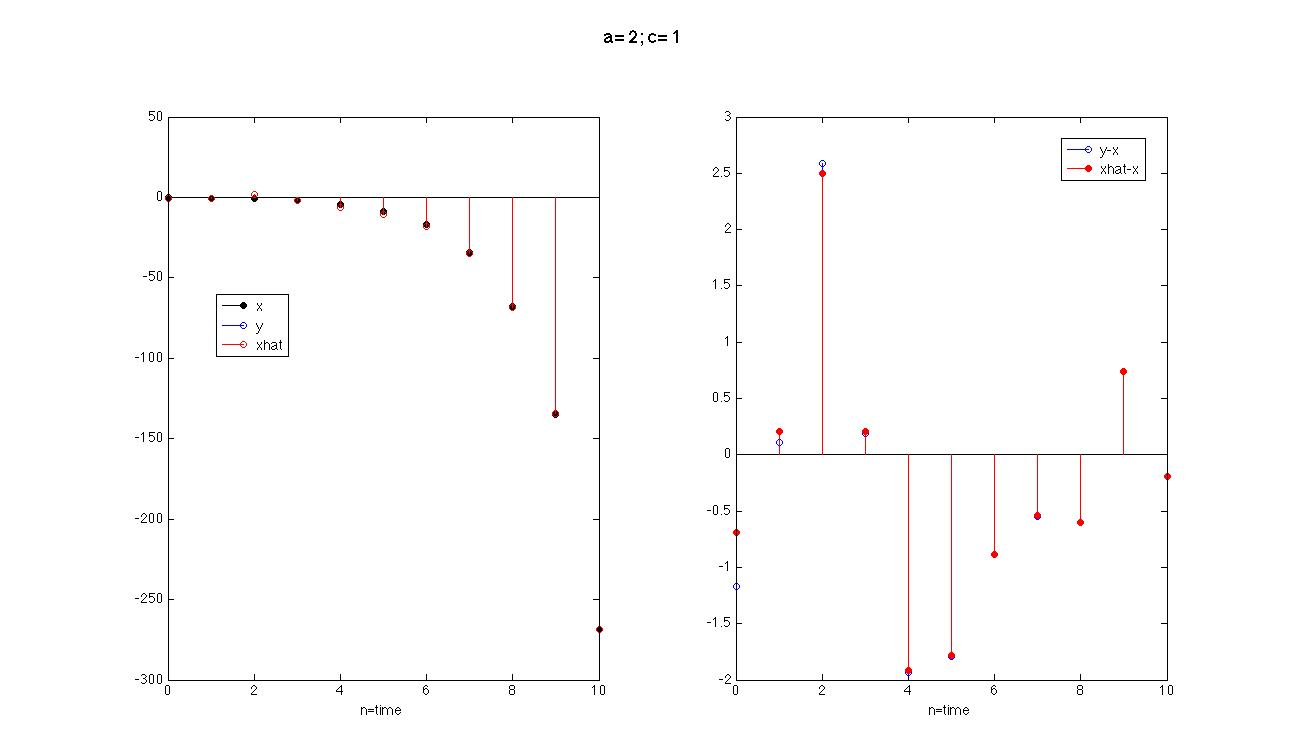
\includegraphics[scale=0.5]{fig1}\\

\textbf{Average bids per contest}: $4\frac{1}{3}$\\

\begin{tabular}{l c l}
Player & \# of bids & Bid dates\\
Aditya Challa & 8 & 5B, 6A, 6B, 7A, 7B, 8A, 9A, 9B\\
Albert Lin & 2 & 9A, 9B\\
Alex Yang & 1 & 5B\\
Andrew Luo & 1 & 1B\\
Anurag Ajay & 3 & 4B, 5B, 6B\\
Arnav Dugar & 7 & 2A, 2B, 3A, 4B, 5B, 6A, 6B\\
Brian Chu & 1 & 3A\\
Chris Dock & 1 & 3B\\
Cong Chen & 1 & 4A\\
Daniel Suryakusuma & 1 & 1B\\
Derek Ahmed & 2 & 9A, 9B\\
Hansong Zhang & 3 & 1B, 2A, 3B\\
Hongling Lu & 8 & 2A, 2B, 3A, 3B, 4A, 4B, 5B, 6A\\
Jong Yun Lee & 1 & 7A\\
Kevin Chen & 1 & 1B\\
Kevin Mawhorter & 1 & 4A\\
Lingtian Cheng & 3 & 2A, 2B, 4B\\
Liuxiao Zhang & 1 & 8A\\
Max Kanwal & 3 & 7A, 7B, 9A\\
Melanie Cebula & 2 & 2B, 4A\\
Myra Haqqi & 12 & 2B, 3A, 3B, 4B, 5B, 6A, 6B, 7A, 7B, 8A, 9A, 9B\\
Viraj Mahesh & 2 & 2A, 3A\\
\end{tabular}\\

Average bids per player: 2.9545\\
After removing the 4 outliers: 1.667\\
Total bid opportunities (contests): 15\\
Fraction: $\frac{1}{5}$ = 0.2\\
Total players: 22\\
Returning players $>$ 1 instance: 12 = only a little over half!\\

\subsection{Interesting observations}
\begin{enumerate}
\item There were no anons. This means people were proud of their work and/or considered themselves strongest players in the class.
\item People corrected each other. Most corrections were done by peers. This means most people weren't afraid of their corrections helping their competitors. Either they're confident their solutions are better and they will also be selected (there is a window of 3 after all) or they don't care because getting the right solution is what matters. 
\item People post close to the deadline. \textcolor{red}{More data needs to be collected.} As the deadline nears, people see that other people haven't posted and are incentivized. They feel there is a greater chance they will be selected. Bids are a deterrence, lack of bids increases \textbf{expected value} which is somehow dependent on time \textcolor{red}{(We should determine what/how correlation)}.
\item There were only 3~4 bids from strong players. Strong bids deterred weak bids. At most 6 bids.
\item Weak players couldn't afford to bid because the cost was too great.
\item As numbers were relatively stable, whether there was an upcoming midterm or a midterm just passed didn't affect number of bids. This could be a negligible effect due to the strength of the bidding players.
\item Exactly 3 players from 2A also participated in 2B. Maybe those 3 players got payoff?
\end{enumerate}

\section{Moving Forward}
\begin{enumerate}
\item Take data from HW solutions (everyone has ALREADY bid) to contrast with Discussion Solutions
\item Flesh out these notes further, check if Questions/Hypothesis are good to explore or if we should explore something else
\item Where in strength do the players lie? Does it match up that they are the strongest players?
\end{enumerate}
\end{document}